
\section{Materiais}

%% Tentar fazer a transição deste slide
%\begin{frame}
%\begin{figure}[]
%	\frametitle{Materiais}
%     \centering
%     \captionsetup{width=\textwidth,font=footnotesize,textfont=bf}   
%     \begin{subfigure}[b]{0.2\textwidth}
% 	\centering
%         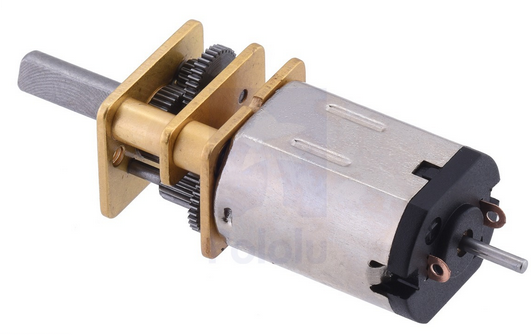
\includegraphics[width=\textwidth,height=\textheight,keepaspectratio]{Figuras/motor.png}
%         \caption{\centering \label{fig:Posicaofinal}}
%     \end{subfigure}
%     \caption{Materiais utilizados}
%    
% \end{figure}
%\end{frame}


\begin{frame}
\vspace{-0.4cm}
\begin{figure}[noframenumbering]
	\frametitle{Materiais}
     \centering
     \captionsetup{width=\textwidth,font=footnotesize,textfont=bf}
     \begin{subfigure}[b]{0.2\textwidth}
 	\centering
         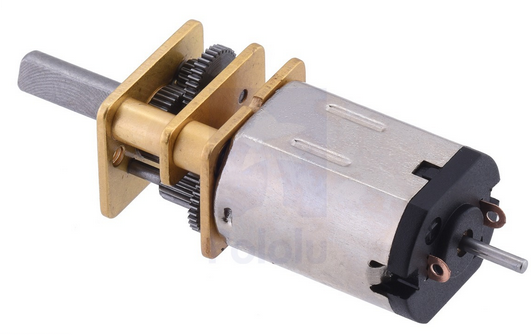
\includegraphics[width=\textwidth,height=\textheight,keepaspectratio]{Figuras/motor.png}
         \caption{\centering \label{fig:Posicaofinal}}
     \end{subfigure}
     ~
     \pause
     \begin{subfigure}[b]{0.2\textwidth}
 	\centering
         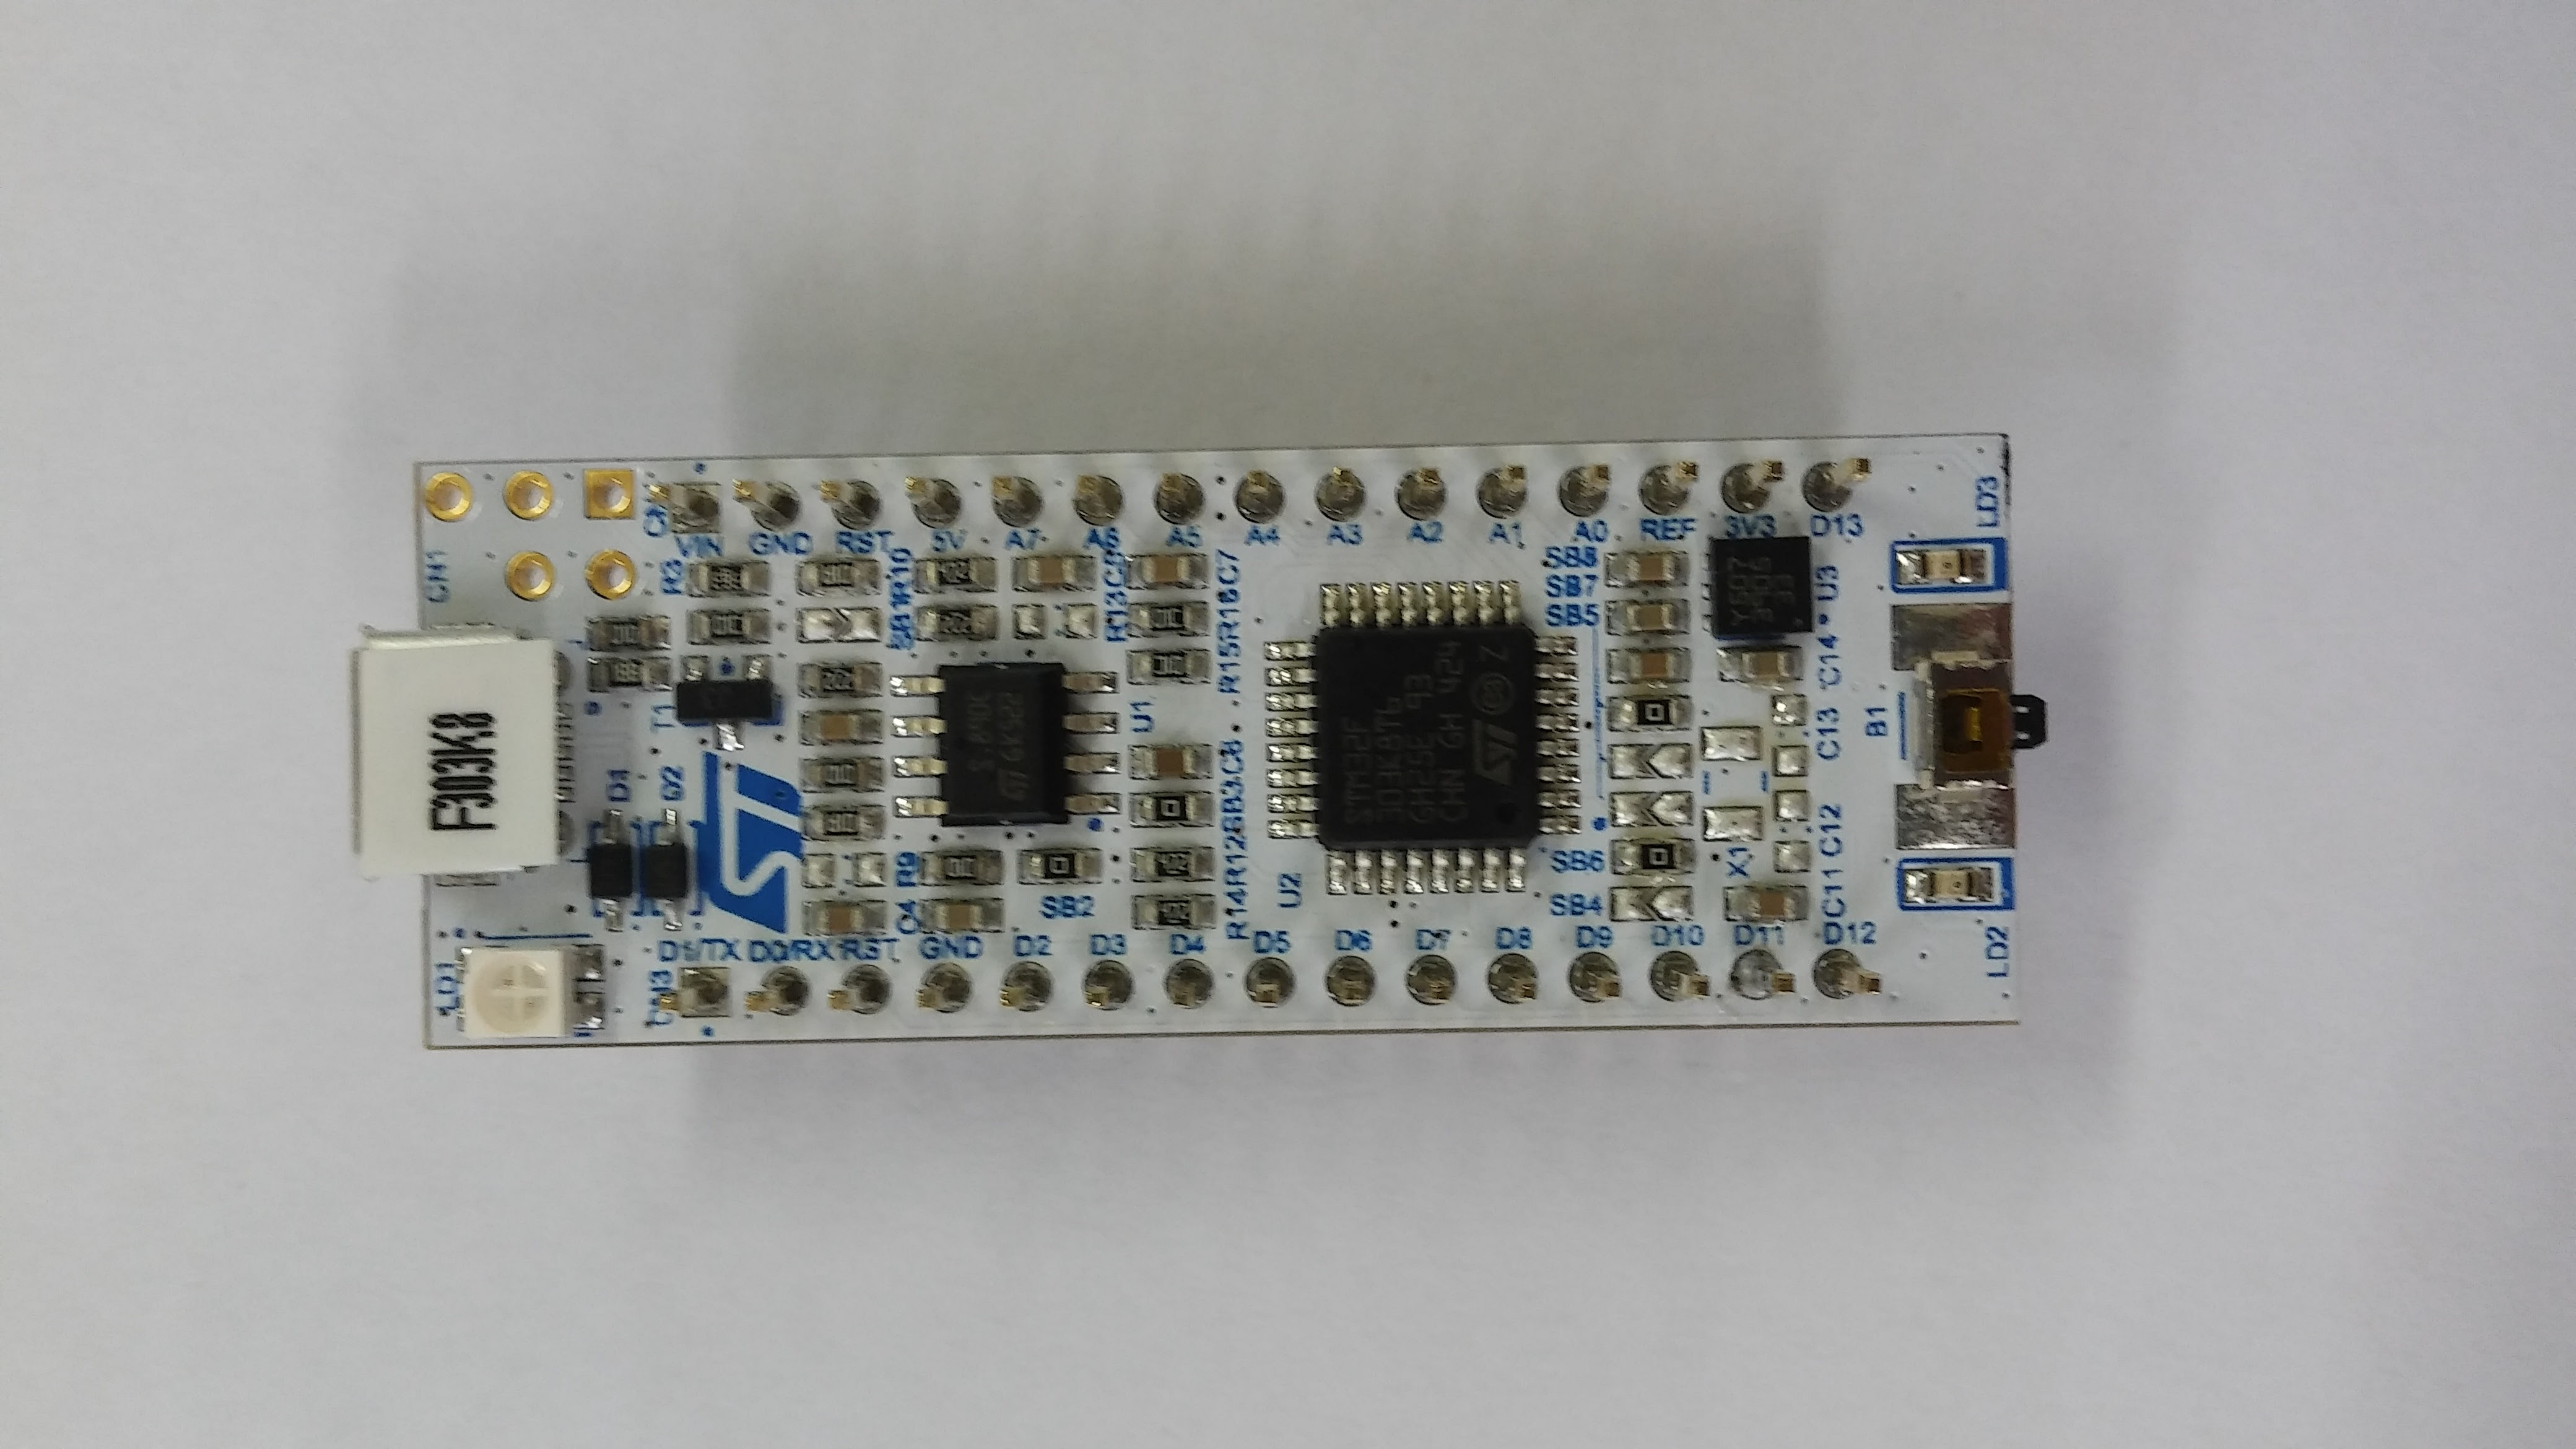
\includegraphics[width=\textwidth,height=0.3\textheight,keepaspectratio]{Figuras/nucleo.jpg}
         \caption{\centering \label{fig:Posicao1}}
     \end{subfigure}
     ~
     \pause
     \begin{subfigure}[b]{0.2\textwidth}
 	\centering
         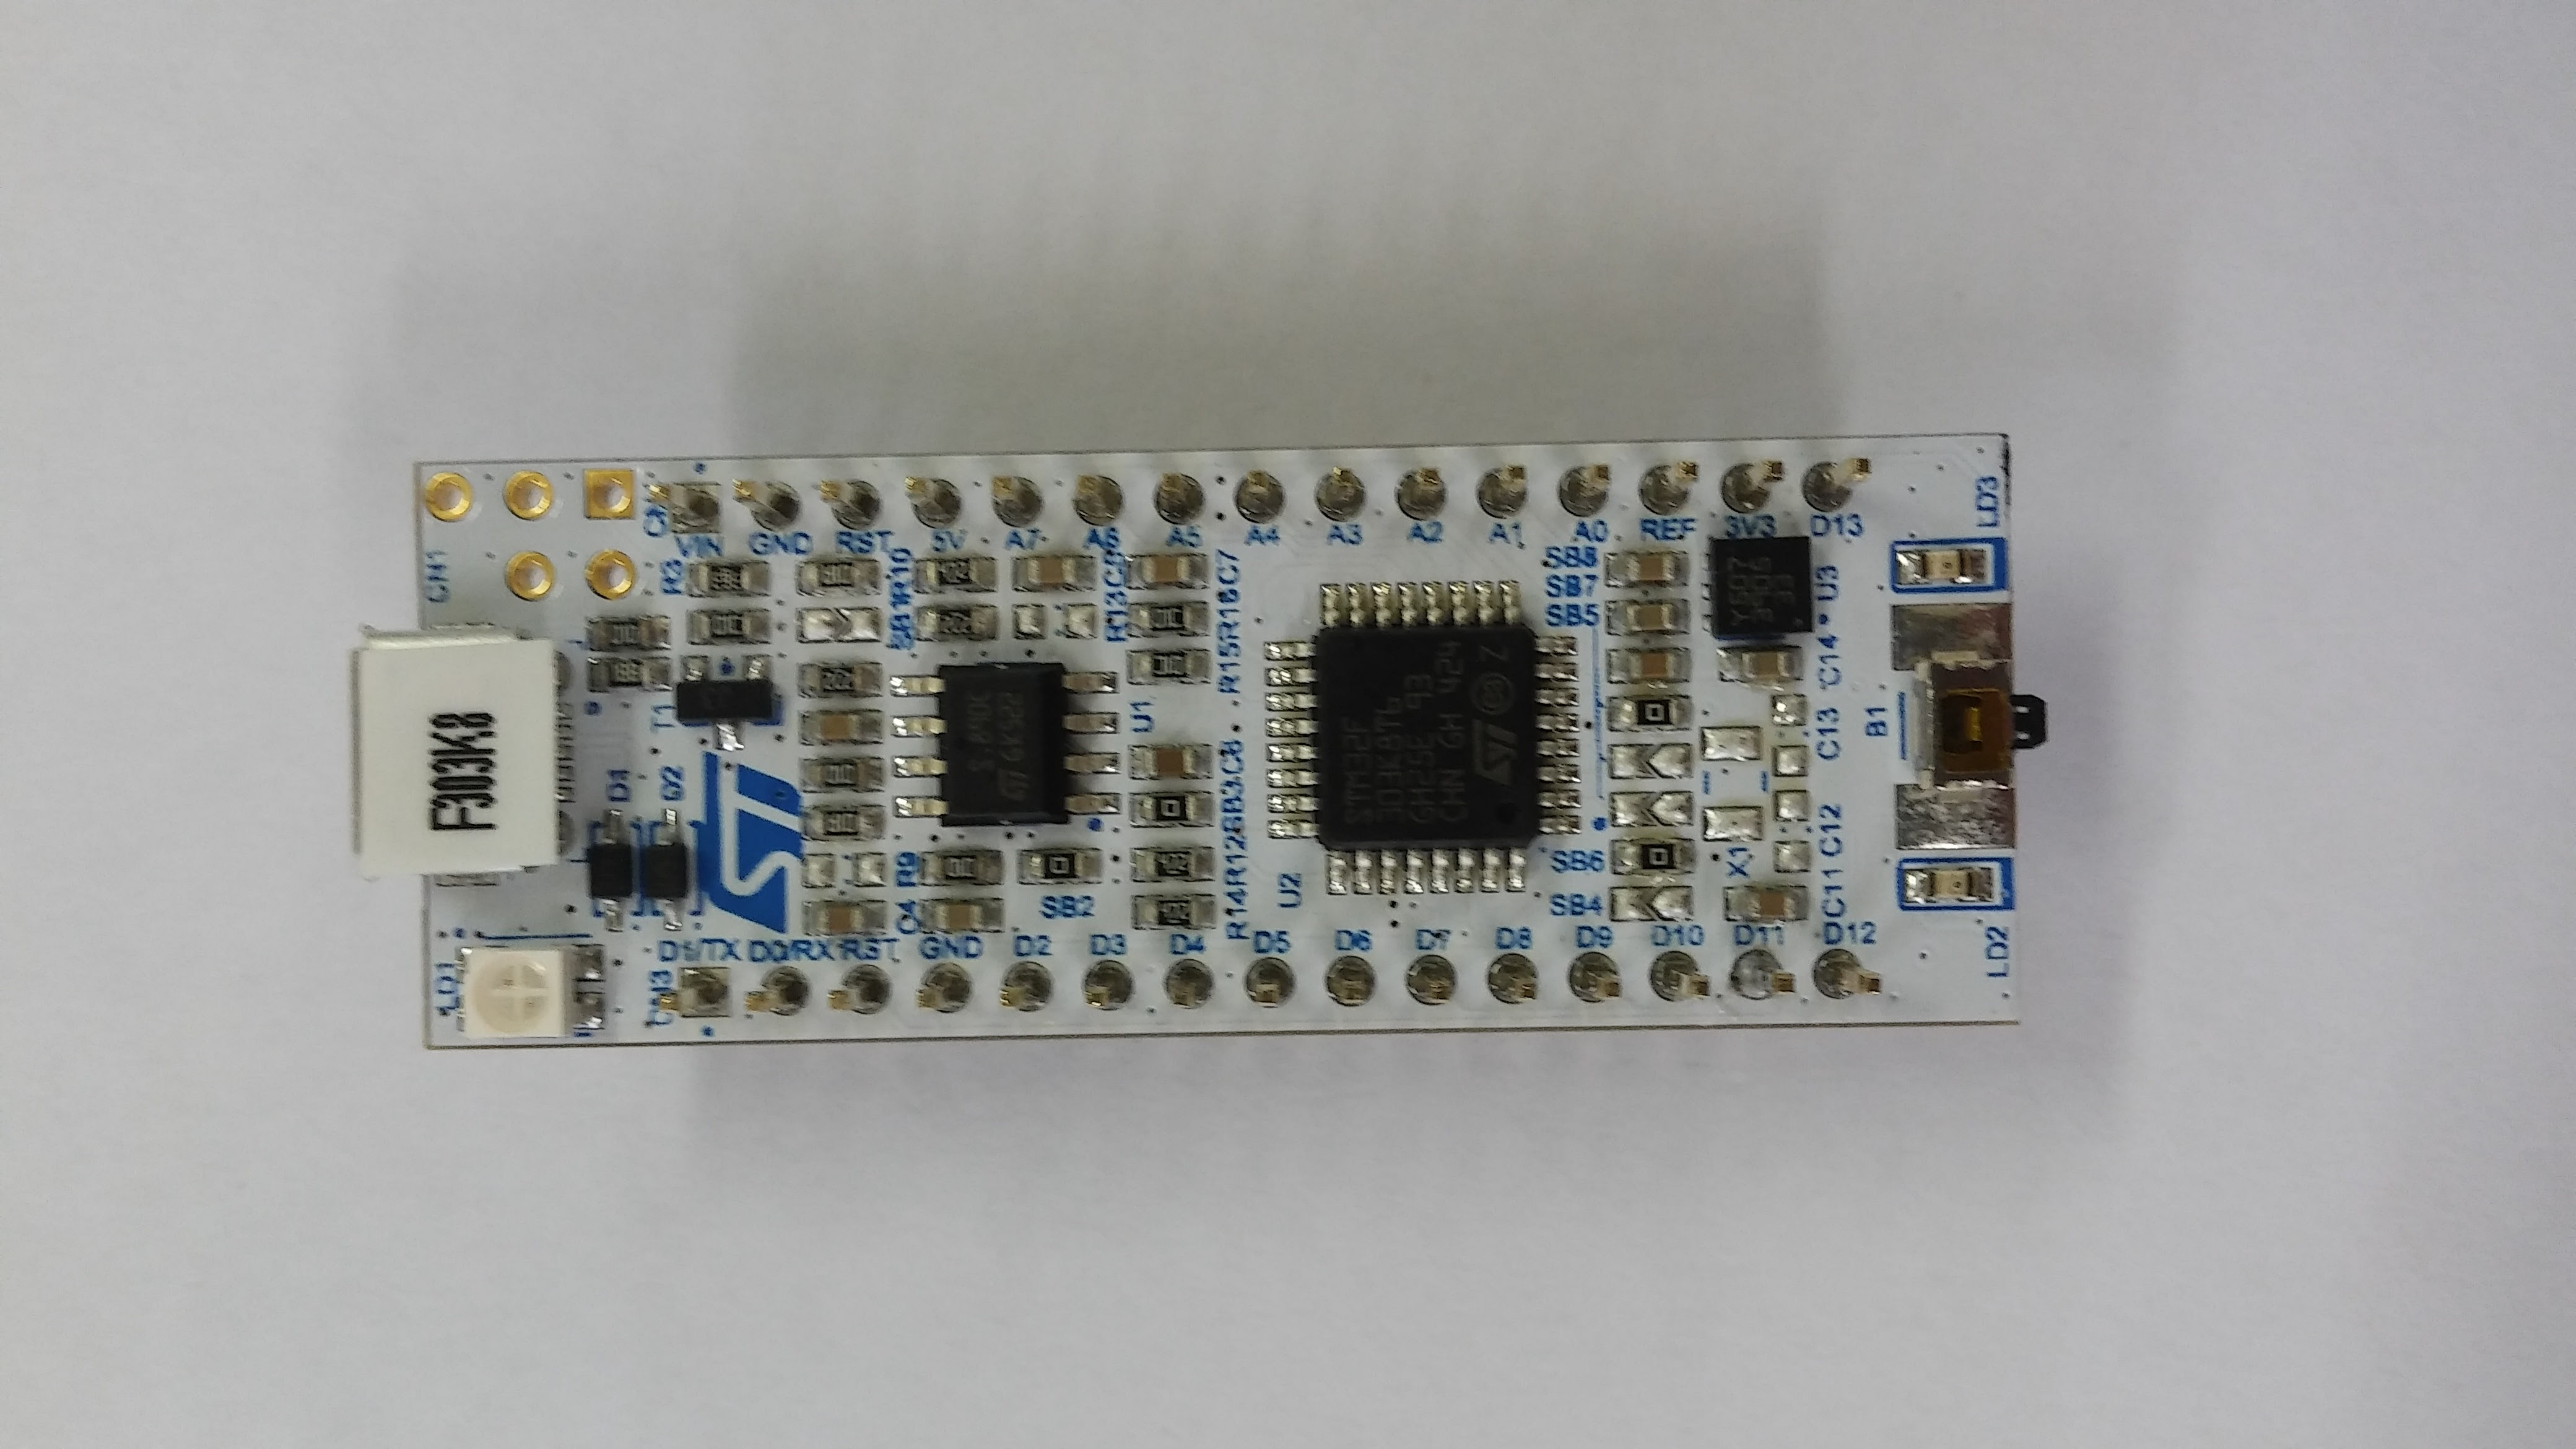
\includegraphics[width=\textwidth,height=0.3\textheight,keepaspectratio]{Figuras/nucleo.jpg}
         \caption{\centering \label{fig:Posicaofjksfjdlkfj}}
     \end{subfigure}
     
     \caption{Materiais utilizados}     
 \end{figure}
\end{frame}

